\chapter{System Requirement and Specification }

\section{Scope of Project}
This project intends to replace the current archaic process of storing health records and the entire insurance policy life cycle i.e. from buying insurance to policy servicing to claim settlement.

The system is based on blockchain technology which helps with decentralized storage of medical records and policy details of every patient. The blockchain technology is basically the combination of three technologies, viz., private key cryptography, P2P network, and program or protocol. The blockchain technology represents an innovation in the field of information registration and distribution that eliminates the need for an intermediate trusted authority to facilitate digital relationships.
        
Blockchain-based systems could help radically improve the insurance industry. But its impact could be much broader. Insurance claims processing and settlement are areas where a customer buys a policy and the policy sets out rules under which one gets coverage. The level of expertise required for claim adjusters or the investigators, who investigate, negotiate and settle claims, varies directly with the nature of loss, under the jurisdiction whose law applies to the contract creation, interpretation and enforcement, one of principal consumer protection issues within the insurance pricing, underwriting, and claim settlement process.
         
Blockchain may be useful in reducing fraud related to the integrity of a policy or claim. By maintaining the integrity of the asset through various owners, Blockchain will minimize counterfeiting, double booking, document or contract alterations. However, use of the Blockchain does not mitigate the risk associated with the majority of first party and third-party frauds. Fraud detection and investigation systems will still be required.
\section{User Classes}
\begin{itemize}
	\item \textbf{User} \newline Citizens of India are going to use the application to access their medical records, give permission to the the requesting parties for their medical records, buying insurance policy, paying premiums and track the status of their claims. The User should have the basic knowledge of using a computer and need to have access to the internet to avail the above mentioned services.
	      	                  
	\item \textbf{Healthcare providers} \newline Healthcare providers have the ability to upload User’s medical records on the blockchain network and view user’s records after permission granted. The personnel using the application needs to have basic knowledge of computers and internet. The Healthcare provider also acts as a node in the blockchain network and thus verify and validate transactions. A network professional is a requirement for the healthcare providers who keeps a checks on the functioning of the node.
	      	                  
	\item \textbf{Insurance Provider} \newline An Insurance Providers provides policy quotations to the User’s, view user’s records after permission granted, grant insurance policies to the user and most importantly settle claims. Basic knowledge of computer and internet is enough. An Insurance Company will also act as a node, verify and validate transactions on the network. A network professional is a requirement for the insurance company who keeps a checks on the functioning of the node.
	      	      
\end{itemize}
\clearpage
\section{Operating Environment}

The software will operate with the following software components and applications:\newline
The software being developed will be running on virtual machines with Linux OS(Ubuntu 16.04). The applications can be accessed with any web browser(Google Chrome, Mozilla Firefox, etc.) on any operating system(Windows, Linux, Mac OS). The users need to have an internet connection to access the applications.

\section{Constraints}
\begin{itemize}
	\item No distributed key generation and management mechanism for recovery of keys provided to user
	\item All of the complex legal terms and conditions of an insurance policy cannot be implemented as a Smart Contract.
	\item There is yet to be found a proper balance between what information about a policy has to be stored on-chain and off-chain.
	\item Automated claim settlement cannot be implemented as a function of a Smart Contract without extensive domain knowledge in order to to cover all of the complex test cases.
\end{itemize}



 


\section{Assumptions and Dependencies}
\textbf{The assumptions are}:
\begin{itemize}
	\item The coding should be error free.
	\item Each person must have an Aadhar Card.
	\item All terms and conditions of a policy agreed between the insurance provider and a client must be understood and encoded as a smart contract.
	\item Constant and stable Internet connection while records are uploaded and claims are settled.
	\item Users must have basic knowledge of interacting with a computer.
\end{itemize}
\textbf{The dependencies are }:
\begin{itemize}
	\item 	The specific hardware and software due to which the product will be run.
	\item   Based on listed requirements and specification the project will be developed and run.
	\item    The end users should have proper understanding of the product.
\end{itemize}
    
\section{External Interface Requirements}
\begin{itemize}
	\item  \textbf{User Interface}:
	      The interfaces for each specific user have been designed so that it is convenient to use. It is a simple and easy to use interface giving more power to the user .The application makes sure at every point, that the User spends most of the time using the application rather than figuring out how to use it.
	      	          
	      The home screen offers a menu with a list of functions that the application performs. The user can select one of the options on the menu, and is taken to the respective page.
	      	          
	\item \textbf{Hardware Interface}: \newline
	      The minimum hardware requirements of a computer running our platform should be:
	      \begin{enumerate}
	      	\item Processor: Processor: 1.8 GHz or faster Dual Core 64-bit 
	      	\item Hard Disk: 512 GB
	      	\item RAM: 4GB or higher
	      	\item OS: Ubuntu 16.04 or higher
	      \end{enumerate}
	      	      
	      The authority nodes are the nodes that maintain the blockchain network and are responsible for verifying and uploading transactions on the network. Therefore, these machines should have, if possible, more computing power than the minimum requirements and a fast and stable internet connection. As the scale of the network increases, the authority nodes will require more computational power.
	\item \textbf{Software Interface}:
	      	      
	      The decentralized applications(DApp) will be hosted on a Virtual Machine that runs Linux Ubuntu 16.04 LTS. The necessary softwares are installed on the nodes running these DApps. Further, these DApps can be accessed using a web browser(eg. Google Chrome, Mozilla Firefox, etc.) on any operating system, be it Windows, Mac or Linux. Any updates for the DApps can be pulled from the respective Github repositories.
	\item \textbf{ Communication Interface:}
	      	      
	      The system requires an internet connection to install new plugins, update already installed ones and the update some of its components (APIs, modules, etc.).
	      	          
	      The file upload and retrieval work on a new protocol i.e. the IPFS protocol which is a protocol built specifically for decentralized file storage and addressing. The IPFS protocol intends to replace HTTP and HTTPS.
	      	         
	      	         
\end{itemize}
\section {System Features}

This section demonstrates the systems most prominent features and explain how they can be used and the results they will give back to the user
\begin{enumerate}
	\item \textbf{User Login}
	   \begin{itemize}
	       \item \textbf{Description \& Priority:} It validates the legitimacy of users i.e. it checks whether the user is registered on the platform or not. This feature has a high priority as without validation users can't use the system.
	       \item \textbf{Stimulus:} Set correct ethereum account in the Metamask extension. The next step is to fill all the login credentials. If all details correct the user will be redirected to the necessary page of the application.
	       \item \textbf{Functional Requirements:} The required software capabilities for this feature are- a web browser and the Metamask browser extension connected to the blockchain network.
	   \end{itemize}
	   %   This feature allows user to be a part of the system. User needs to provide the necessary details and if all details fulfill the requirements the user is provided a unique pair of public and private keys. This key pair will be further used in the other features of the system.
	\item \textbf{Upload Medical Record}
	   %   This feature is only available for the healthcare providers. The healthcare providers will generate medical reports and bills of the patient(user) and then upload it on the IPFS servers. The IPFS returns a unique hash of the record uploaded and this particular hash is encrypted with the user’s public key in-order to maintain user privacy.
	    \begin{itemize}
	       \item \textbf{Description \& Priority:} The feature is available only to the hospitals. The medical records generated by the hospital for a user are electronically stored using this feature. It has a medium priority as the users can be a part of the system but might not have any medical records associated with them. 
	       \item \textbf{Stimulus:} Enter the user's Aadhaar number and other fields in the form. When clicked on submit, user's PGP key-pair is fetched from the IPFS and the records are encrypted and stored on the IPFS. All the metadata of the records is stored on blockchain.
	       \item \textbf{Functional Requirements:} The required software capabilities for this feature are- a web browser and the Metamask browser extension connected to the blockchain network.
	   \end{itemize}
	\item \textbf{Deploy Policy}
	   %   This is most crucial feature of the system. This feature handles all the intricacies of the insurance system. It allows the valid users to view policy details put up by the insurance provider, select policies, grant record access permissions to the insurance providers, choose the policy after comparing the quotations sent by the insurance providers and pay premiums for the policies as per the conditions. The insurance providers on the other hand just analyze user’s medical records and send policy quotations to the user. The rest other functionalities are handled by the smart contract in the blockchain network.
	   	    \begin{itemize}
	       \item \textbf{Description \& Priority:} Allows insurance companies on the platform to deploy policy templates as smart contracts. The deployed templates provides user all details about a policy. Only insurance companies have access to this feature. It has high priority as without this feature the insurance companies will be futile.   
	       \item \textbf{Stimulus:} Enter the policy coverage and the name of the policy. Once clicked on submit, the policy template is deployed and it's mapped against the insurance company in the organization smart contract.
	       \item \textbf{Functional Requirements:} The required software capabilities for this feature are- a web browser and the Metamask browser extension connected to the blockchain network.
	   \end{itemize}   	      
	\item \textbf{Apply Policy}
	   %   This feature allows the claims to be settled against the hospital bills and medical reports tagged as claimable. The entire process is automated. The smart contracts analyze the bills and medical records uploaded by the healthcare providers. If all the conditions in the user’s policy contract match with those of the medical records then the smart contract will settle the claim and necessary amount is transferred into the user’s account. Here, the insurance providers are not required to do any work and thus saving valuable time of the involved parties.
	   \begin{itemize}
	       \item \textbf{Description \& Priority:} Allows users to buy insurance policy from the available list of policy templates. The priority is medium as a user on the platform may/may not buy insurance policy.   
	       \item \textbf{Stimulus:} Select insurance company from the drop-down list. Once selected, list of all policies offered by the insurance companies are displayed. Click on apply button against the policy name to buy that policy. A Metamask notification pops-up which makes the user pay 1 ether(this amount is refunded when the insurance company accepts the policy). Next, the user is directed to share medical records page. User can either share records at that time or later. 
	       \item \textbf{Functional Requirements:} The required software capabilities for this feature are- a web browser and the Metamask browser extension connected to the blockchain network.
	   \end{itemize}   	      
\end{enumerate}
\section{Tools and Technologies Used}
\begin{enumerate}
	\item \textbf{Parity Ethereum}
	      	      
	      It is an open-source software for building the decentralized Web. Parity Develops cutting-edge blockchain technologies to foster innovations. Parity Ethereum provides the core infrastructure essential for the speedy and reliable services. It uses Proof of
	      Authority consensus protocol. It provides clean, modular code base for easy customization along with minimal memory and storage footprint. The entire information about Parity is available on wiki.parity.io. 
	   %   Geth is an alternative which uses Proof of Work mechanism which high intensive mathematical calculations and uses a lot of electricity as all the nodes try to verify the transactions at the same time whereas in Proof of Authority allows only one node to verify a particular transaction and other just validate it.
	      	               
	\item \textbf{Solidity}
	      	      
	      Solidity is a contract-oriented, high-level language for implementing smart contracts. It was influenced by C++, Python and JavaScript and is designed to target the Ethereum Virtual Machine (EVM). Ethereum only uses solidity to write smart contracts so there is no other choice of programming smart contracts other than solidity.
	      	      
	\item \textbf{Web3.js}
	      	      
	      Web3.js is a collection of libraries which allow you to interact with a local or remote ethereum node, using a HTTP or IPC connection. It helps the frontend interact with the blockchain.
	      	      
	\item  \textbf{React JS}
	
	      ReactJS is a JavaScript library for building user interfaces. It is maintained by Facebook and a community of individual developers and companies.React allows developers to create large web applications which can change data, without reloading the page. The main purpose of React is to be fast, scalable, and simple. It works only on user interfaces in application.ReactJS is one of the most widely used libraries to build frontend in blockchain based applications and other web applications.It’s community support is very strong in relations to blockchain.
	      \clearpage
	\item   \textbf{MySQL}
	
    	MySQL is an Oracle-backed open source relational database management system (RDBMS) based on Structured Query Language (SQL). MySQL runs on virtually all platforms, including Linux, UNIX and Windows. Although it can be used in a wide range of applications, MySQL is most often associated with web applications and online publishing.
        MySQL is based on a client-server model. The core of MySQL is MySQL server, which handles all of the database instructions (or commands). MySQL server is available as a separate program for use in a client-server networked environment and as a library that can be embedded (or linked) into seperate applications. 
        %  Everytime a policy contract changes its state to Active, the user application server inserts an entry into a MySQL database specifying address of the node that has setup the transaction and the address of the contract on which the transaction has to be performed.

\item   \textbf{MongoDB}

	MongoDB is a cross-platform and open-source document-oriented database, a kind of NoSQL database. As a NoSQL database, MongoDB shuns the relational database’s table-based structure to adapt JSON-like documents that have dynamic schemas which it calls BSON. 
    This makes data integration for certain types of applications faster and easier. MongoDB is built for scalability, high availability and performance from a single server deployment to large and complex multi-site infrastructures.
    % Every miner has a listener setup at their machines and if the MySQL entry matches their address, then they schedule a transaction to run a later date. In order to persistence of these transactions even in case of server crash, or shutdown due to maintenance all scheduled transactions are stored in a MongoDB collection.


	      	      
\end{enumerate}

\clearpage
\section{Design}
\subsection{System Architecture}
\begin{figure}[h!]
	\centering
	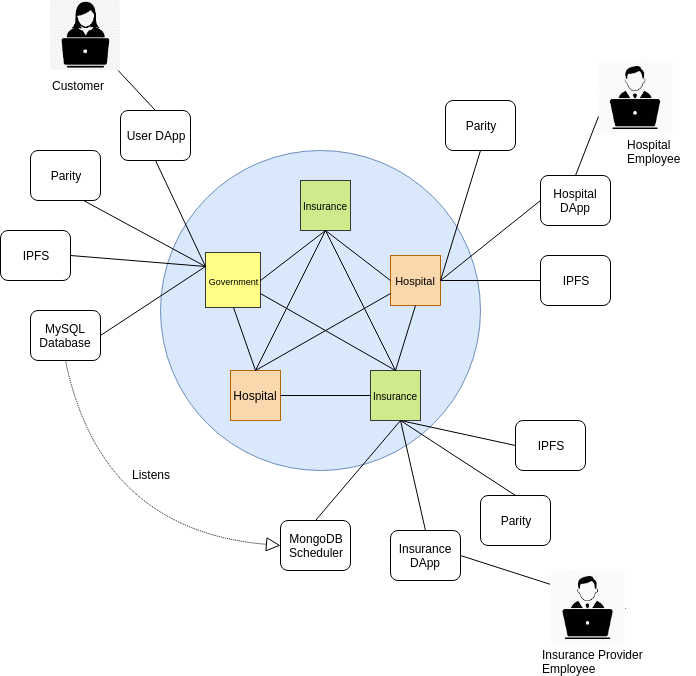
\includegraphics[width=\linewidth]{Images/SystemArchitecture.png}
	\caption{System Architecture}
	%\label{fig:SystemArchitecture}
\end{figure} 

The system architecture has 5 main blocks-
\begin{enumerate}
	\item 	\textbf{User Application Block:} This block shows the interface for the user and what functionalities are available to the users. The users perform four functions - store the public and private keys that they receive on joining the system, view and grant access permissions to the medical records, view and buy the insurance policies and then pay premiums for the policies bought.
	\\
	\item \textbf{Healthcare Provider Block:} The healthcare provider has two functions to perform- create medical records and upload those records on the file server available.
	\item \textbf{Inter-Planetary File System(IPFS):} This block tells about the functions performed by the IPFS. It has two functions - storing medical records at appropriate node and generating an appropriate IPFS hash for the uploaded medical record. This hash will help to access the file stored on these servers.
	\item \textbf{Insurance Provider Block:} This block tells the functionalities of the insurance company. It has three functions available to perform- give policy quotations to the user, access user’s medical records after permission granted by the user and settle claims using smart contracts.
	\item \textbf{Blockchain Block:} This block shows the underlying technology being used to implement the system. The blockchain is collections of transactions stored in blocks in a specific manner. The transactions stores the necessary data - like medical record data, smart contracts,etc. The data stored in the transaction is stored in hex value.
\end{enumerate}

\section{Policy State Diagram}
\begin{figure}[!h]
	\centering
	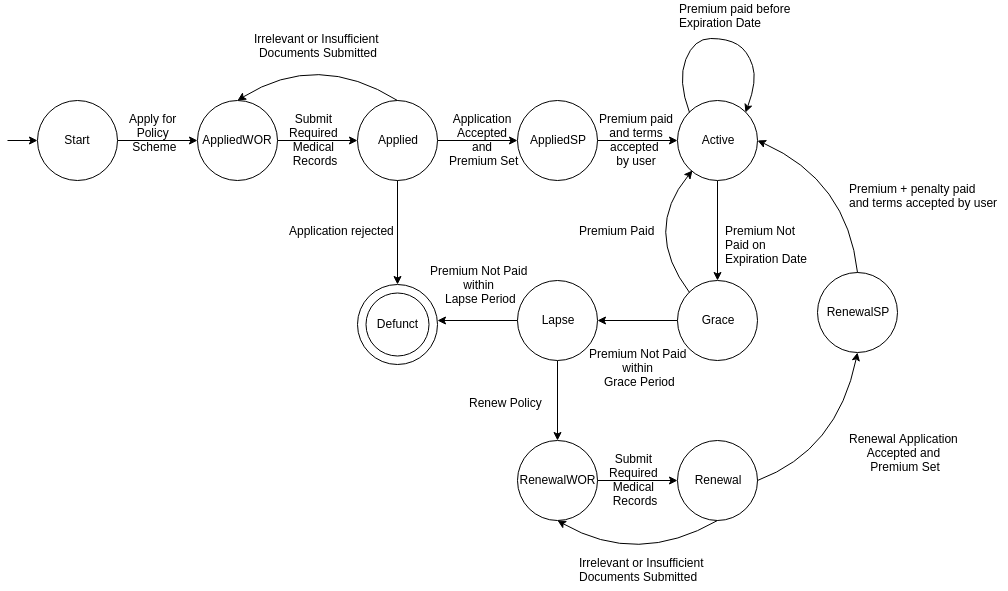
\includegraphics[width=\linewidth]{Images/PolicyStateDiagram.png}
	\caption{Policy State Diagram}
	%\label{fig:SystemArchitecture}
\end{figure} 

A policy smart contract on our platform can be equated to a Non-deterministic Finite Automata (NFA). The above diagram depicts the following states and conditions necessary for state transitions:

\begin{enumerate}
    \item \textbf{AppliedWOR} : After a customer/user applies for a policy scheme, a new smart contract is instantiated, and the initial state of the newly instantiated smart contract is Applied without records (AppliedWOR) and the state isn’t updated till the user submits his/her medical records.
    
    \item \textbf{Applied} : Once all the necessary medical records the state of the policy changes to Applied. A Third Party Administrator (TPA) will verify the submitted medical records. If the submitted records are not sufficient or relevant then the TPA can revert the state of the policy contract back to AppliedWOR. If the submitted records are valid and sufficient, then the TPA approves the application and sets a premium. The TPA might reject the application in case of a pre-existing condition.
    
     \item  \textbf{AppliedSP} : The state of policy changes to AppliedSP after the premium is set by a TPA.

 \item  \textbf{Active} : After the user has accepted the terms and conditions of the policy and pays the premium set by the TPA, the policy state changes to Active. If the user pays his policy premium before it’s expiration date, then the policy continues to remain in Active state.

 \item \textbf{Grace} : If the user does not pay his/her premium before the due date, then the policy state is changed to Grace. The due date for the user to pay his/her premium is extended by a month, if the user makes the payment within this period then the state is updated to Active again.

 \item \textbf{Lapse} : If the user does not make the payment before the new due date then state of the policy changes to Lapse. The user has a six month period from the date of policy lapse to renew or the policy goes to defunct state.

 \item \textbf{RenewalWOR} : If the user decides to renew his policy after it has lapsed, then he applies for the policy again and the state of the policy changes to Renewal without records.

 \item \textbf{Renewal} : Once all the necessary medical records the state of the policy changes to Renewal. A Third Party Administrator (TPA) will verify the submitted medical records. If the submitted records are not sufficient or relevant then the TPA can revert the state of the policy contract back to RenewalWOR.
 
\item \textbf{RenewalSP} : If the submitted records are valid and sufficient, then the TPA approves the application and sets a premium and a penalty. Once the user pays the premium and penalty set by the TPA, the state of the policy changes back to Active.

 \item \textbf{Defunct} : If the user does not renew his/her policy within six months of the policy lapsing, then the policy state changes to Defunct. 

\end{enumerate}


\section{Encryption Process}
\begin{figure}[!h]
	\centering
	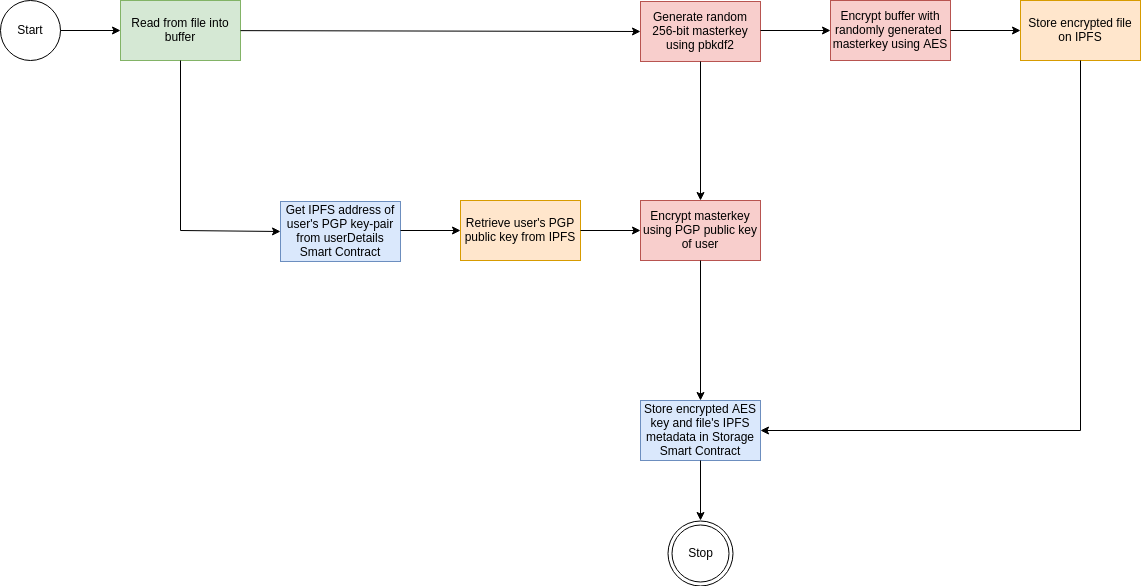
\includegraphics[width=\linewidth]{Images/Encryption.png}
	\caption{Encryption}
	%\label{fig:SystemArchitecture}
\end{figure} 

All medical records for a patient are uploaded on a distributed and immutable file system known as \textbf{Interplanetary File System} (IPFS). The metadata of these records being stored on IPFS are stored to reduce storage load on and also to decrease latency of data retrieval from the blockchain network. Before a record is stored on IPFS it is encrypted such that it can be accessed only by the owner of the record or whoever they decide to share access with. \\ The following steps are performed in the encryption process :
\begin{enumerate}
   \item The record to be uploaded is read and stored in a buffer.
   \item A call is made to the userDetails Smart Contract to get IPFS address of the user’s PGP key-pair file.
   \item The PGP key file of the user is retrieved from IPFS.
   \item A 256-bit master key is generated randomly using \textbf{pbkdf2}.
   \item The buffer containing contents of the record is encrypted using \textbf{Advanced Encryption Standard (AES)}. 
   \item The randomly generated master key is then itself encrypted using PGP public key of the user retrieved from IPFS.
   \item The buffer is then stored on IPFS and the IPFS hash of the newly stored file and the encrypted master key along with some other metadata about the file is stored in the Storage Smart Contract. 
\end{enumerate}
\section{Decryption Process}
\begin{figure}[!b]
	\centering
	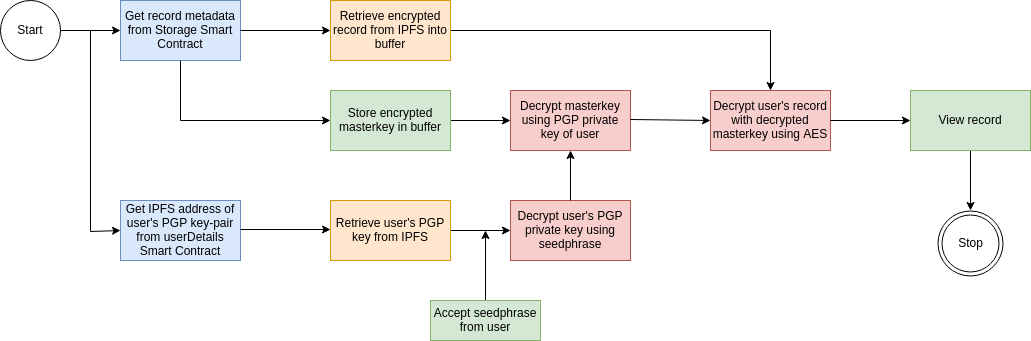
\includegraphics[width=\linewidth]{Images/Decryption.png}
	\caption{Decryption}
	%\label{fig:SystemArchitecture}
\end{figure} 

In order for the owner or a permitted entity to view a medical record, its metadata has to be fetched from the smart contract and after selecting the record to view the file has to be fetched from the Interplanetary File System (IPFS) and decrypted. The following steps are performed in the decryption process :
Metadata of all records owned by a user or those records he/she has permitted access is fetched from Storage Smart Contract and displayed.
\\
\begin{enumerate}
    \item The user enters his/her seedphrase.
    \item Once a record is selected to be viewed the IPFS address user’s PGP key pair is fetched from UserDetails Smart Contract.
    \item The encrypted record and the user’s PGP key is fetched from IPFS.
    \item The encrypted PGP private key of the user is unlocked with the seedphrase. If the seedphrase is incorrect, it results in an error.
    \item The encrypted masterkey is decrypted using the unlocked PGP private key.
    \item Finally, the medical record is decrypted using the decrypted masterkey and displayed to the user.  
\end{enumerate}


\clearpage
\section{UML Diagrams}
\subsection{Use Case Diagram}
\begin{figure}[h!]
	\centering
	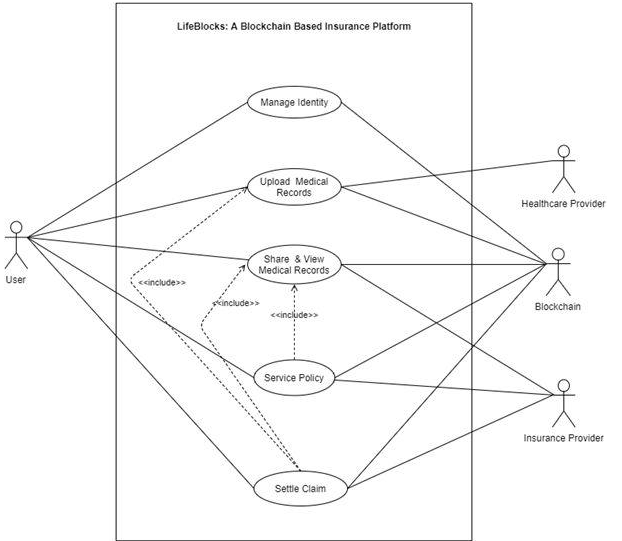
\includegraphics[width=\linewidth]{Images/Usecase.jpg}
	\caption{Use Case Diagram}
	%\label{fig:Use Case}
\end{figure}

\textbf{Use Case Description}
\begin{enumerate}
	\item \textbf{Manage Identity } \\
	      \textbf{ Identifier: DIP1} \\
	      \textbf{ Description:} 
	      Users provide Aadhaar Card to authenticate themselves and once validated the blockchain will generate their public-private keys.\\
	      \textbf{Goal:}
	      \begin{enumerate}
	      	\item  Verify the user.
	      	\item  Generate public-private keys.
	      	\item  Allows users to use the platform.
	      \end{enumerate}
	      \textbf{Preconditions} No Preconditions
	      \textbf{Assumptions}
	      \begin{enumerate}
	      	\item Aadhaar database is reliable.
	      \end{enumerate}
	      \textbf{Frequency :} One time verification and key generation for every user.
	      	                  
	      	                  
	      \textbf{Basic Course}
	      \begin{enumerate}
	      	\item	User authenticates themselves by providing their Aadhaar Card.
	      	\item	Blockchain verifies the Aadhaar against the Aadhaar Database.
	      	\item	Once validated successfully, unique public-private key pair is generated.
	      \end{enumerate}
	      \textbf{Actors}
	      \begin{enumerate}
	      	\item  User
	      	\item Blockchain
	      \end{enumerate}
	      	                  
	\item \textbf{Upload Medical Records } \\
	      \textbf{ Identifier: DIP2} \\
	      \textbf{ Description:} User goes to the hospital for medical examination and the records generated are uploaded by the hospital after encrypting those records using the user’s public key thus maintain record privacy.
	      	              
	      \textbf{Goal:}
	      \begin{enumerate}
	      	\item  Securely upload medical records on the network.
	      	\item  Users are the sole owners of their medical records.
	      \end{enumerate}
	      \textbf{Preconditions} Healthcare provider should have user’s Aadhaar Number.
	      	      
	      \textbf{Assumptions}
	      \begin{enumerate}
	      	\item Aadhaar database is reliable.
	      \end{enumerate}
	      \textbf{Frequency :} Multiple times for each user.\\
	      \textbf{Basic Course}
	      \begin{enumerate}
	      	\item	User authenticates themselves by providing their Aadhaar Card.
	      	\item	Medical checkup is completed and medical records are generated.
	      	\item	User provides aadhaar number and hospital encrypts record using that public key.
	      	\item 	Hospital uploads signed records on blockchain network.
	      	      	      	      
	      \end{enumerate}
	      \textbf{Actors}
	      \begin{enumerate}
	      	\item  User
	      	\item Healthcare provider
	      	\item Blockchain
	      \end{enumerate}
	      	         
	\item \textbf{Share and View Medical Records} \\
	      \textbf{ Identifier: DIP3} \\
	      \textbf{ Description:} Once medical records generated, user is the sole owner of the medical records and can share the records with either insurance or healthcare providers as and when required. For this the user changes the access list of the medical records.
	      	      
	      \textbf{Goal:}
	      \begin{enumerate}
	      	\item  Securely share medical records with insurance or healthcare providers.
	      \end{enumerate}
	      \textbf{Preconditions} Users have their public key.\\
	      \textbf{Assumptions}
	      \begin{enumerate}
	      	\item Aadhaar database is reliable.
	      \end{enumerate}
	      \textbf{Frequency :} Multiple times by each user.
	      User has a medical record.
	      	                  
	      \textbf{Basic Course}
	      \begin{enumerate}
	      	\item	User changes access list of medical record by adding the public key of the entity with whom they wish to share their records.
	      	\item	Blockchain verifies the Aadhaar against the Aadhaar Database.
	      	\item	Once permission given the accessing party can view the records.
	      \end{enumerate}
	      \textbf{Actors}
	      \begin{enumerate}
	      	\item User
	      	\item Blockchain
	      	\item Insurance Provider
	      	\item Healthcare Provider
	      \end{enumerate} 
	      	                  
	\item \textbf{Service Policy} \\
	      \textbf{Identifier: DIP4} \\
	      \textbf{Description:} User wants to buy an insurance policy and thus sends an application for the same to the insurance provider. The insurance provider verifies the medical records of the user and if valid the insurance policy is awarded to the user.
	      	                      
	      \textbf{Goal:} 	Award insurance policy to the user.
	   %   \begin{enumerate}
	   %   	\item  
	   %   \end{enumerate}
	      \textbf{Preconditions} Users have their public key.
	      \newline
	      \textbf{Assumptions} No Assumption.
	   %   \begin{enumerate}
	   %   	\item 
	   %   \end{enumerate}
	      \textbf{Frequency :} Multiple times for each user.\newline
	      \textbf{Basic Course}
	      \begin{enumerate}
	      	\item	Users apply for insurance policy and share their medical records with the insurance provider.
	      	\item	Insurance providers receive the application and send quotes.
	      	\item  	Insurance providers verify user’s health records and if valid they award the insurance policy.
	      	\item 	User’s pay premiums for the policy.
	      \end{enumerate}
	      \textbf{Actors}
	      \begin{enumerate}
	      	\item User
	      	\item Blockchain
	      	\item Insurance Provider
	      \end{enumerate} 
	      \textbf{Include}
	      \begin{enumerate}
	      	\item Share and View Medical Records(DIP3)
	      \end{enumerate} 
	      	              
	\item \textbf{Settle Claim} \\
	      \textbf{Identifier: DIP5} \\
	      \textbf{Description:} In case of a claimable event, the healthcare provider uploads the necessary medical records of the user on the blockchain. The smart contracts analyze the medical records and if all conditions met the claim is settled.
	      	      
	      	                      
	      \textbf{Goal:} 		
	      	      
	      \begin{enumerate}
	      	\item  Get medical treatment.
	      	\item  Upload new medical records.
	      \end{enumerate}
	      \textbf{Preconditions} Users have their public key.
	      \newline
	      \textbf{Assumptions}
	      \begin{enumerate}
	      	\item 
	      \end{enumerate}
	      \textbf{Frequency :}  Multiple times for each user per insurance policy.\newline
	      \textbf{Basic Course}
	      \begin{enumerate}
	      	\item	Occurrence of a claim event (like medical treatment or death).
	      	\item	Hospital uploads medical records (DIP3) in case of medical treatment (DIP2) or death certificate (DIP3) in case of death of the user.
	      	\item  	Insurance providers verify user’s health records and if valid they award the insurance policy.
	      	\item 	User’s pay premiums for the policy.
	      \end{enumerate}
	      \textbf{Actors}
	      \begin{enumerate}
	      	\item User
	      	\item Blockchain
	      	\item Healthcare Provider
	      	\item Insurance Provider
	      \end{enumerate} 
	      \textbf{Include}
	      \begin{enumerate}
	      	\item Upload Medical Records (DIP2)
	      	\item Share and View Medical Records(DIP3)
	      \end{enumerate}     
\end{enumerate}
\clearpage
\textbf{Class Diagram}
\begin{figure}[!h]
	\centering
	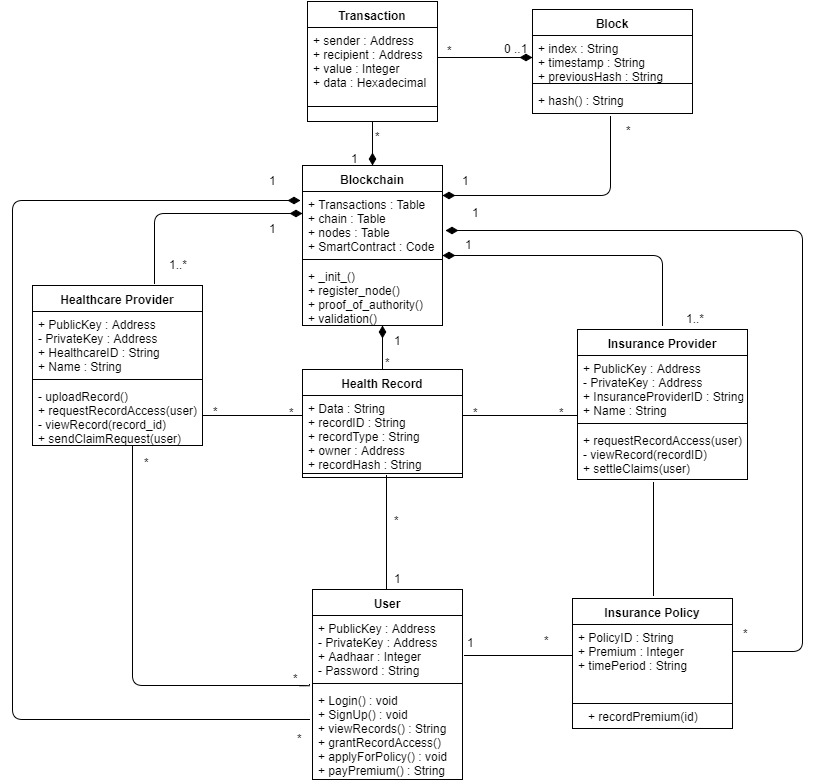
\includegraphics[width=\linewidth]{Images/UML/ClassDiagram.jpg}
	\caption{ Class Diagram}
	%\label{fig:Use Case}
\end{figure}
\clearpage
\textbf{Sequence Diagram}
\begin{figure}[!t]
	\centering
	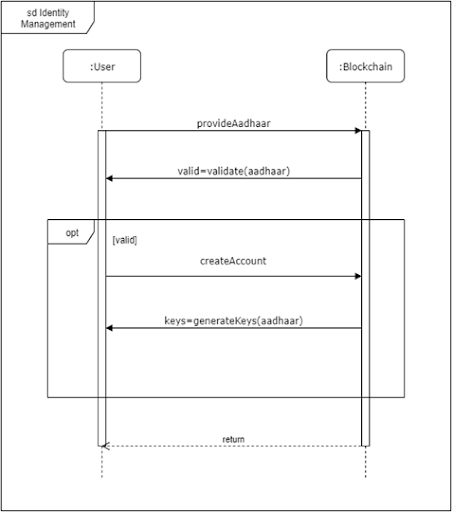
\includegraphics[width=0.6\linewidth]{Images/UML/SequenceIdentityManagement.png}
	\caption{ Sequence Identity Management}
	%\label{fig:Use Case}
\end{figure}
\begin{figure}[!b]
	\centering
	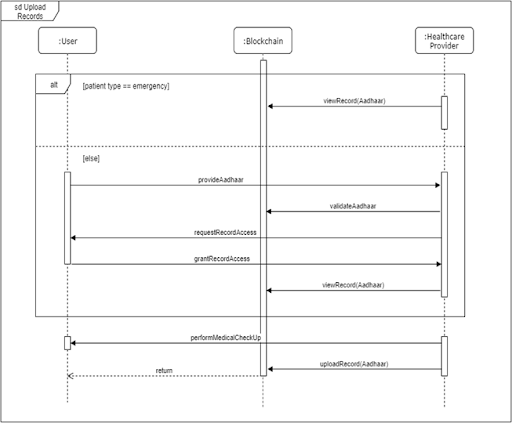
\includegraphics[width=0.6\linewidth]{Images/UML/SequenceEHRStorage.png}
	\caption{ Sequence EHR Storage}
	%\label{fig:Use Case}
\end{figure}
\begin{figure}[!t]
	\centering
	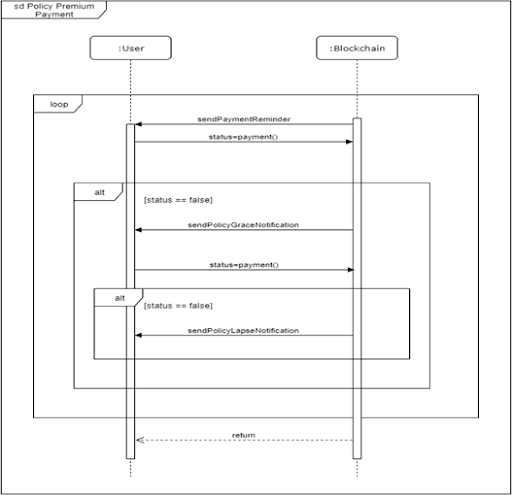
\includegraphics[width=0.7\linewidth]{Images/UML/SequencePolicyPremiumPayment.png}
	\caption{ Sequence Policy Premium Payment}
	%\label{fig:Use Case}
\end{figure}
\begin{figure}[!b]
	\centering
	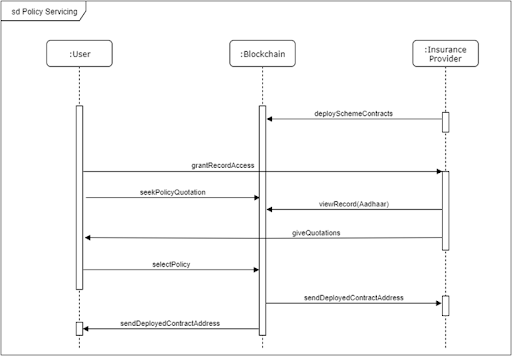
\includegraphics[width=0.7\linewidth]{Images/UML/SequencePolicyServicing.png}
	\caption{ Sequence Policy Servicing}
	%\label{fig:Use Case}
\end{figure}
\clearpage
% \begin{figure}[!t]
% 	\centering
% 	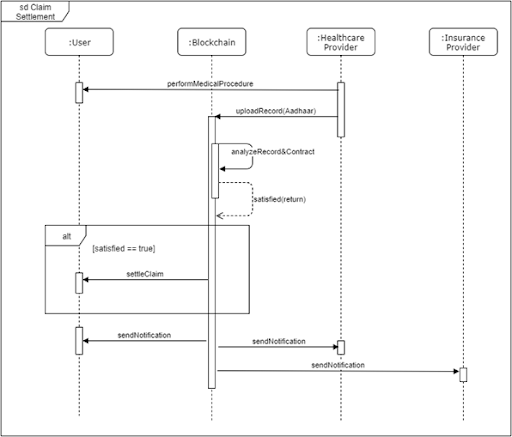
\includegraphics[width=0.6\linewidth]{Images/UML/SequenceClaimSettlement.png}
% 	\caption{ Sequence Claim Settlement}
% 	\label{fig:Use Case}
% \end{figure}
\textbf{Activity Diagram}
\begin{figure}[!h]
	\centering
	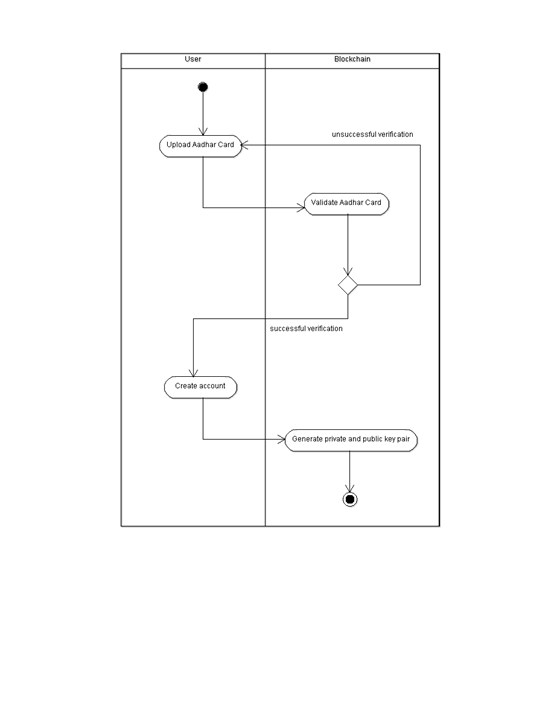
\includegraphics[width=\linewidth]{Images/UML/ActivityIdentityManagement.png}
	\caption{ Activity Identity Management}
	%\label{fig:Use Case}
\end{figure}
\begin{figure}
	\centering
	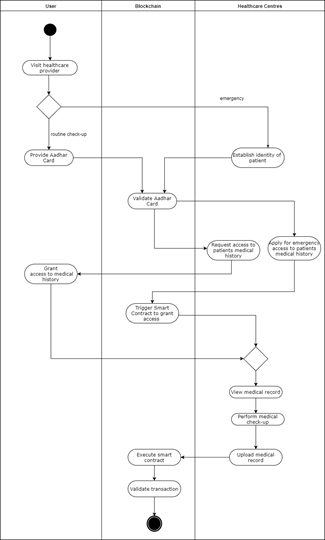
\includegraphics[width=.8\linewidth]{Images/UML/ActivityEHRStorage.png}
	\caption{ Activity EHR Storage}
	%\label{fig:Use Case}
\end{figure}
\begin{figure}
	\centering
	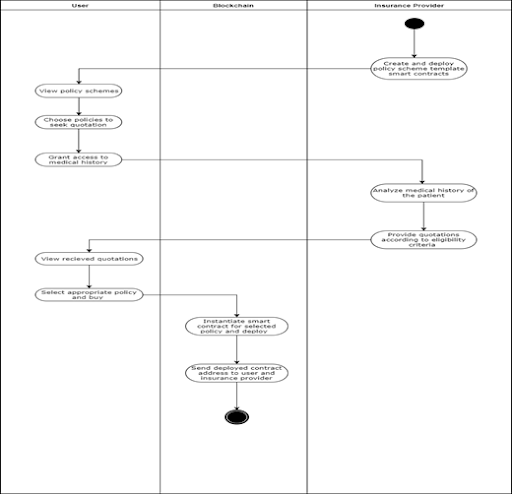
\includegraphics[width=.8\linewidth,height=15cm]{Images/UML/ActivityPolicyServicing.png}
	\caption{ Activity Policy Servicing}
	%\label{fig:Use Case}
\end{figure}

% \begin{figure}
% 	\centering
% 	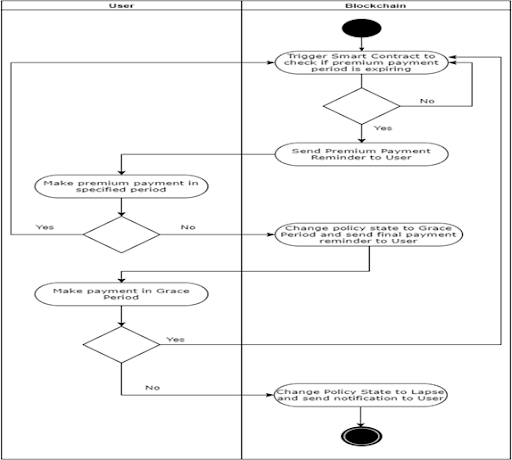
\includegraphics[width=0.6\linewidth,height=10cm]{Images/UML/ActivityPolicyPremiumPayment.png}
% 	\caption{ Sequence Claim Settlement}
% 	\label{fig:Use Case}
% \end{figure}
